% !TeX spellcheck = en_US
\subsection{Thermodynamic Perturbation\label{Sec:FEM:TP}}
Thermodynamic Perturbation (TP), also known as Free Energy Perturbation (FEP), exponential average, or Zwanzig equation, was developed by Zwanzig,\cite{ZwanzigJCP1954} and Landau and Lifshitz, independently, and probably by Peierls\cite{JorgensenJCTC2008}. 

A reference system containing $N$-particles can be described by Hamiltonian $H_{0}(\mathbf{x},\mathbf{p}_{x})$, which is a function of $3N$ Cartesian coordinates, $\mathbf{x}$, and their conjugated momenta, $\mathbf{p}_{x}$. Similarly, the target system can be described by Hamiltonian $H_{1}(\mathbf{x},\mathbf{p}_{x})$. These two systems are related by 
\begin{equation}
  H_{1}(\mathbf{x},\mathbf{p}_{x}) = H_{0}(\mathbf{x},\mathbf{p}_{x}) + \Delta H (\mathbf{x},\mathbf{p}_{x})
  \label{Eq:FEM:TP:deltaH}
\end{equation}
The Helmholtz free energy difference between the target and the reference systems, $\Delta A$, can be given in terms of the ratio of the corresponding partition functions, $Q_{1}$ and $Q_{0}$:
\begin{equation}
  \Delta A  =  -\frac{1}{\beta}\ln\frac{Q_{1}}{Q_{0}},
  \label{Eq:FEM:TP:deltaA}
\end{equation}
where $\beta = {(k_{B}T)}^{-1}$, and
\begin{equation}
  Q_i = \frac{1}{{h}^{3N}N!} \iint \exp\left[-\beta H_i(\mathbf{x},\mathbf{p}_{x})\right] \diff\mathbf{x}\diff \mathbf{p}_\mathbf{x}.
  \label{Eq:FEM:TP:PF}
\end{equation}
Taking Eq.~\ref{Eq:FEM:TP:PF} into Eq.~\ref{Eq:FEM:TP:deltaA}, we obtain
\begin{align}
  \Delta A  =&  -\frac{1}{\beta}\ln{\frac{\iint \exp\left[-\beta H_{1}(\mathbf{x},\mathbf{p}_{x})\right] \diff\mathbf{x}\diff\mathbf{p}_\mathbf{x}}{\iint \exp\left[-\beta H_{0}(\mathbf{x},\mathbf{p}_{x}) \right] \diff\mathbf{x}\diff\mathbf{p}_\mathbf{x}}}\\
            =& -\frac{1}{\beta}\ln{\frac{\iint \exp\left[-\beta \Delta H(\mathbf{x},\mathbf{p}_{x})\right] \exp\left[-\beta H_{0}(\mathbf{x},\mathbf{p}_{x})\right] \diff\mathbf{x}\diff\mathbf{p}_\mathbf{x}}{\iint \exp\left[-\beta H_{0}(\mathbf{x},\mathbf{p}_{x})\right] \diff\mathbf{x}\diff\mathbf{p}_\mathbf{x}}},
  \label{Eq:FEM:TP:deltaA2}
\end{align}
The probability density function of finding the reference system in a state defined by positions $\mathbf{x}$ and momenta $\mathbf{p}_{x}$ is 
\begin{equation}
  P_{0}(\mathbf{x},\mathbf{p}_{x}) = \frac{ \exp[-\beta H_{0}(\mathbf{x},\mathbf{p}_{x}) ] }{\iint \exp[-\beta H_{0}(\mathbf{x},\mathbf{p}_{x}) ] \diff\mathbf{x}\diff\mathbf{p}_\mathbf{x}}
  \label{Eq:FEM:TP:proden}
\end{equation}
If the probability density function is used, Eq.~\ref{Eq:FEM:TP:deltaA2} becomes
\begin{equation}
  \Delta A = -\frac{1}{\beta} \ln \iint \exp[-\beta \Delta H(\mathbf{x},\mathbf{p}_{x})] P_{0}(\mathbf{x},\mathbf{p}_{x}) \diff\mathbf{x}\diff\mathbf{p}_\mathbf{x},
  \label{Eq:FEM:TP:deltaA3}
\end{equation}
or, equivalently,
\begin{equation}
  \Delta A = -\frac{1}{\beta} \ln{\langle \exp{\left[-\beta \Delta H(\mathbf{x},\mathbf{p}_{x})\right]} \rangle_{0}},
  \label{Eq:FEM:TP:deltaA4}
\end{equation}
Here, $\left \langle \cdots \right \rangle _{0}$ denotes an ensemble average over configurations sampled from the reference state. Equation~\ref{Eq:FEM:TP:deltaA4} is the basic equation of TP. It states that $\Delta A$ can be estimated by sampling only equilibrium configurations of the reference state.

Note that integration over the kinetic term in the partition function, Eq.~\ref{Eq:FEM:TP:PF}, can be carried out analytically. Thus, it cancels out in Eq.~\ref{Eq:FEM:TP:deltaA}, and Eq.~\ref{Eq:FEM:TP:deltaA4} becomes
\begin{equation}
  \Delta A_f = -\frac{1}{\beta} \ln{\left< \exp(-\beta \Delta U) \right>_{0}},
  \label{Eq:FEM:TP:deltaA5}
\end{equation}
where $\Delta U$ is the difference in the potential energy between the target and the reference states. The subscript $f$ is an indication of a forward ($0\rightarrow 1$) TP calculation. The integration implied by the statistical average is now carried out over particle coordinates only. The variance of $\Delta A$ is
\begin{equation}
    \delta^2 \Delta A_f=\frac{1}{N_0\beta^2}\left(\frac{\left<(\exp(-\beta \Delta U))^2\right>_0}{\left(\left<\exp(-\beta \Delta U)\right>_0\right)^2}-1\right).
\end{equation}

If we exchange the reference and the target systems, and repeat the same derivation, using the same convention for $\Delta A$ and $\Delta U$ as before, we have a backward TP expression for the free energy difference
\begin{equation}
  \Delta A_b = \frac{1}{\beta} \ln{ \left \langle \exp(\beta \Delta U) \right \rangle_{1}},
  \label{Eq:FEM:TP:deltaA6}
\end{equation}
and the variance is
\begin{equation}
  \delta^2 \Delta A_b=\frac{1}{N_1\beta^2}\left(\frac{\left<(\exp(\beta \Delta U))^2\right>_1}{\left(\left<\exp(\beta \Delta U)\right>_1\right)^2}-1\right).
\end{equation}
Although expressions Eq.~\ref{Eq:FEM:TP:deltaA5} and Eq.~\ref{Eq:FEM:TP:deltaA6} are formally equivalent, their convergence properties may be quite different. This means that there is a preferred direction to carry out the required transformation between the two states. One should start the perturbation from the state having larger important region in phase space. In other words, the reference system should be the one with higher entropy, and the transformation should proceed in the direction in which the entropy decreases. If we have the free energy differences from both the forward and backward TP calculations, we can compute the ``best estimate'' of $\Delta A$ as
\begin{equation}
    \Delta A = \frac{(\delta^2 \Delta A_f)^{-1}\Delta A_f+(\delta^2 \Delta A_b)^{-1}\Delta A_b}{(\delta^2 \Delta A_f)^{-1}+(\delta^2 \Delta A_b)^{-1}},
\end{equation} 
with variance
\begin{equation}
    \delta^2 \Delta A=\frac{1}{(\delta^2 \Delta A_f)^{-1}+(\delta^2 \Delta A_b)^{-1}}.
\end{equation} 

Since $\Delta A$ is calculated as the average over a quantity that depends only on $\Delta U$, this average can be computed over probability distribution $P_0(\Delta U)$ instead of $P_{0}(\mathbf{x},\mathbf{p}_{x})$. Then, $\Delta A$ in Eq.~\ref{Eq:FEM:TP:deltaA3} can be expressed as a one-dimensional integral over energy difference
\begin{equation}
  \Delta A = -\frac{1}{\beta} \ln \int \exp(-\beta \Delta U) P_{0}(\Delta U) \diff\Delta U,
  \label{Eq:FEM:TP:deltaA7}
\end{equation}
If $U_{0}$ and $U_{1}$ were functions of a sufficient number of identically distributed random variable, $\Delta U$ would follow a Gaussian distribution, which is a consequence of the central limit theorem. In practice, the probability distribution $P_{0}(\Delta U)$ deviates somewhat from an ideal Gaussian case, but still has a ``Gaussian-like'' shape. This indicates that the value of the integral in Eq.~\ref{Eq:FEM:TP:deltaA7} depends on the low-energy tail of the distribution. Using the language of Jarzynski for the nonequilibrium work\cite{JarzynskiPRE2006}, the maximum of $P_0(\Delta U)$ is the typical energy difference, and the peak value of $P_0(\Delta U)\cdot \exp{(-\beta \Delta U)}$ is the dominant realization that contributes the most to $\Delta A$. It clearly shows in Fig.~\ref{Fig:TP:Pdistribution} that the dominant realization lies to the left of the typical one.

\begin{figure}[htbp]
	\centering
	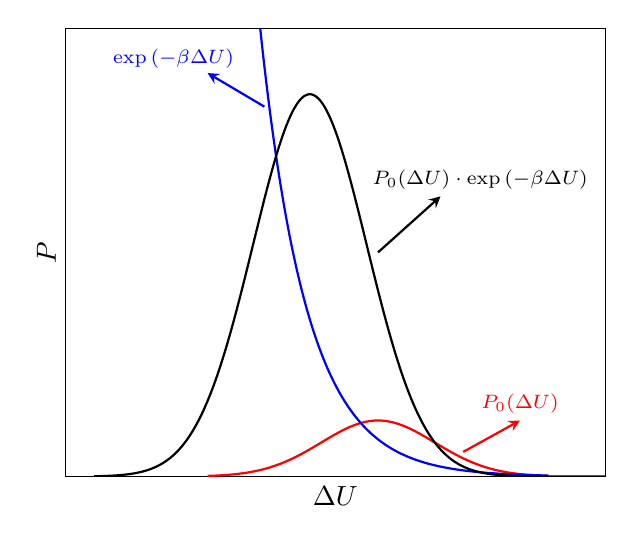
\begin{tikzpicture}
	\def\lims{xmin=-6.5,xmax=3,ymin=0.0,ymax=40}
	\begin{axis}[\lims,
	xtick=\empty, ytick=\empty, minor tick num=0, 
	xlabel=$\Delta U$,
	ylabel={$P$},
	%ytick={0,10,...,40},
	]
	% use TeX as calculator:
	\addplot[thick,color=red,domain=-4:2,samples=500] {5*exp(-(x+1)*(x+1)/2)};
	\addplot[thick,color=blue,samples=500,domain=-4:2] {exp(-1.2*x)};
	\addplot[thick,color=black,samples=500,domain=-6:3] {exp(-1.2*x)*5*exp(-(x+1)*(x+1)/2)};
	\draw[thick,red,->,>=stealth] (axis cs:0.5,2.2) to (axis cs:1.5,5.0);
	\draw[thick,blue,->,>=stealth] (axis cs:-3,33) to (axis cs:-4,36);
	\draw[thick,black,->,>=stealth] (axis cs:-1,20) to (axis cs:0.1,25);
	\draw[red] (axis cs:1.5,6.5) node{\scriptsize$P_0(\Delta U)$};
	\draw[blue] (axis cs:-4.6,37.3) node{\scriptsize$\exp{(-\beta \Delta U)}$};
	\draw[black] (axis cs:0.8,26.5) node{\scriptsize$P_0(\Delta U)\cdot \exp{(-\beta \Delta U)}$};
	\end{axis}
	\end{tikzpicture}
	\caption{$P_{0}(\Delta U)$, the Boltzmann factor $\exp(-\beta \Delta U)$ and their product, which is the integrand in Eq.~\ref{Eq:FEM:TP:deltaA7}. The low-$\Delta U$ tail of the integrand is poorly sampled with $P_{0}(\Delta U)$ and, therefore, is known with low statistical accuracy. However, it provides an important contribution to the integral.}\label{Fig:TP:Pdistribution}
\end{figure}

%\begin{figure}[htbp]
%	\centering
%	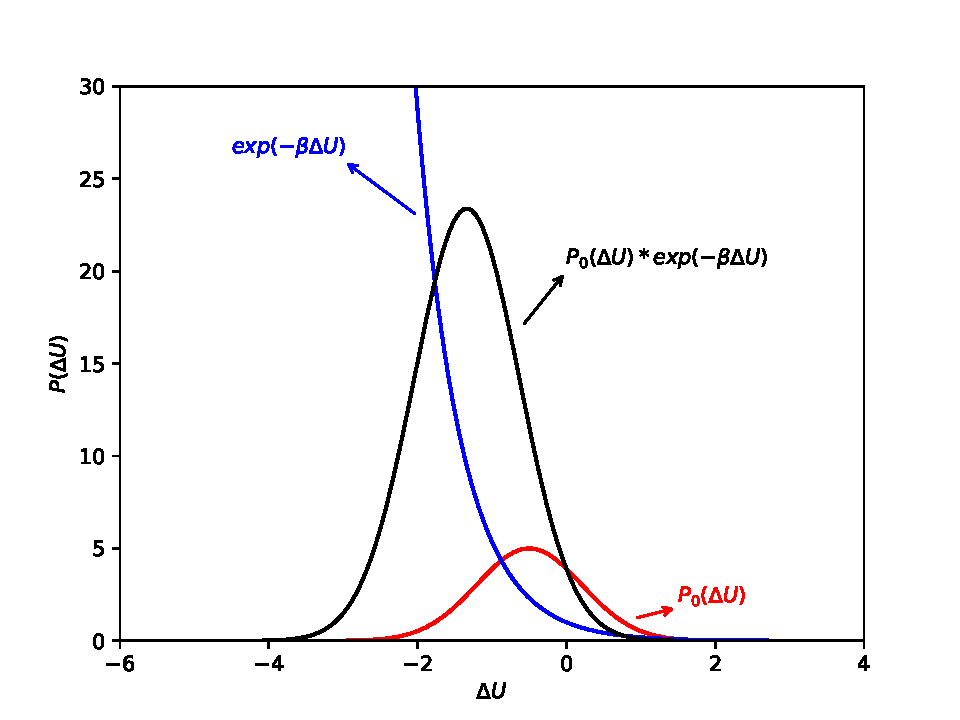
\includegraphics[width=0.6\textwidth]{figures/TP.pdf}\\
%\caption{$P_{0}(\Delta U)$, the Boltzmann factor $\exp(-\beta \Delta U)$ and their product, which is the integrand in \ref{Eq:FEM:TP:deltaA7}. The low-$\Delta U$ tail of the integrand is poorly sampled with $P_{0}(\Delta U)$ and, therefore, is known with low statistical accuracy. However, it provides an important contribution to the integral.}\label{Fig:TP:Pdistribution}
%\end{figure}
Even though $P_{0}(\Delta U)$ is only rarely an exact Gaussian, it is instructive to consider this case in more detail. If we substitute
\begin{equation}
  P_{0}(\Delta U) = \frac{1}{\sqrt{2\pi}\sigma}\exp{\left[-\frac{(\Delta U - \left \langle \Delta U \right \rangle_{0})^2}{2\sigma^2}\right]}
  \label{Eq:FEM:TP:gaussian}
\end{equation}
where
\begin{equation}
  \sigma^2 = \left \langle \Delta U^2 \right \rangle_{0} - \left \langle \Delta U \right \rangle_{0}^2
  \label{Eq:FEM:TP:variance}
\end{equation}
to Eq.~\ref{Eq:FEM:TP:deltaA7}, we obtain
\begin{equation}
  \exp(-\beta \Delta A) = \frac{C}{\sqrt{2\pi}\sigma} \int \exp{\left[-\frac{(\Delta U - \left \langle \Delta U \right \rangle_{0} + \beta \sigma ^2)^2}{2\sigma^2}\right]} \diff\Delta U
  \label{Eq:FEM:TP:expdeltaA}
\end{equation}
Here, $C$ is independent of $\Delta U$
\begin{equation}
  C = \exp{\left[-\beta \left(\left \langle \Delta U \right \rangle_{0} - \frac{1}{2} \beta \sigma ^2\right)\right]}
  \label{Eq:FEM:TP:C}
\end{equation}
If $P_{0}(\Delta U)$ is Gaussian, the integral in Eq.~\ref{Eq:FEM:TP:expdeltaA} can be evaluated analytically using cumulant expansion (see appendix~\ref{chapter:Appendix:CE})
\begin{equation}
  \Delta A = \left< \Delta U \right>_{0} - \frac{1}{2} \beta \sigma ^2.
  \label{Eq:FEM:TP:deltaA8}
\end{equation}
If the distribution of $\Delta U$ deviates from Gaussian, there will be extra terms measuring the skewness of Gaussian. With the leading term, $\Delta A$ becomes
\begin{equation}
  \Delta A = \left< \Delta U \right>_{0} - \frac{1}{2} \beta \sigma ^2 + \frac{\beta^2}{6} \left(\left<\Delta U^3\right>_0-3\left<\Delta U^2\right>_0\left<\Delta U\right>_0+2\left<\Delta U\right>_0^3\right).
  \label{Eq:FEM:TP:deltaA9}
\end{equation}
%The overlap matrix\cite{KlimovichJCAMD2015} is a useful metric in characterizing the magnitude of overlap in the phase space. It is recommended to be used as a consistency check, as in the case of the TP-based methods. If the weight of each of the $N$ samples $x_{n}$ (collected from all $K$ states) in the $i$th state as:
%\begin{equation}
%W_{n,i}(x_{n}) = \frac{e^{\beta G_{i} - \beta U_{i}(x_{n})}}{\sum_{k=1}^{K} N_{k}e^{\beta G_{k}-\beta U_{k}(x_{n})}}
%\label{Eq:FEM:TP:weights}
%\end{equation}
%Then, the overlap matrix is a $K \times K$ matrix with entries:
%\begin{equation}
%O_{i,j} = \sum_{n=1}^{N}\frac{N_{i} e^{\beta G_{i} - \beta U_{i}(x_{n})}}{\sum_{k=1}^{K} N_{k}e^{\beta G_{k}-\beta U_{k}(x_{n})}}\frac{e^{\beta G_{j} - \beta U_{j}(x_{n})}}{\sum_{l=1}^{L} N_{l}e^{\beta G_{l}-\beta U_{l}(x_{n})}}
%\label{Eq:FEM:TP:om}
%\end{equation}

In 2002, Jarzynski proposed a generalized free energy perturbation method termed ``targeted free energy perturbation''.\cite{JarzynskiPRE2002} This method generalizes the free energy perturbation method between two states, $A$ and $B$, by introducing an intermediate state $A^\prime(\mathbf{y})$ by mapping $\mathcal{M}$ from the microstate of the system $\mathbf{x}$ to another one $\mathbf{y}$ in the configuration space or phase space
\begin{equation}
	\mathcal{M}: \mathbf{x} \to \mathbf{y}(\mathbf{x}),
\end{equation}
The potential energy function of the mapped state $A^\prime(\mathbf{y})$ is
\begin{equation}
	U_{A^\prime}(\mathbf{y})=U_A(\mathbf{x})+\beta^{-1}\ln J(\mathbf{x}),
\end{equation}
where $J(\mathbf{x})=|\partial \mathbf{y}/\partial \mathbf{x}|$ is the Jacobian of the mapping $\mathcal{M}$. The Helmholtz free energy difference between state $A$ and state $A^\prime$ is zero by noticing that
\begin{align*}
	\Delta F_{A^\prime A}=&-\beta^{-1}\ln\frac{Z_{A^\prime}}{Z_A}\notag\\
	                     =&-\beta^{-1}\ln \frac{\int e^{-\beta U_{A^\prime}(\mathbf{y})}\diff y}{Z_A}\notag\\
	                     =&-\beta^{-1}\ln \frac{\int e^{-\beta (U_{A^\prime}(\mathbf{y})-U_A(\mathbf{x}))}e^{-\beta U_A(\mathbf{x})}\diff y}{Z_A}\notag\\
	                     =&-\beta^{-1}\ln \frac{\int J^{-1}(\mathbf{x})e^{-\beta U_A(\mathbf{x})}\diff y}{Z_A}\notag\\
	                     =&-\beta^{-1}\ln \frac{\int e^{-\beta U_A(\mathbf{x})}\diff x}{Z_A}\notag\\
	                     =&0.
\end{align*}
The calculation of the free energy difference between state $A$ and state $B$ can be replaced by the calculation of free energy difference between state $A^\prime$ and state $B$. The latter can be written as
\begin{align}
	\Delta F_{BA^\prime}=&-\beta^{-1}\ln {\int e^{-\beta (U_B(\mathbf{y})-U_{A^\prime}(\mathbf{y}))}\rho_{A^\prime}(\mathbf{y})\diff \mathbf{y}}\notag\\
	                    =&-\beta^{-1}\ln {\int e^{-\beta \Phi(\mathbf{x})}\rho_{A}(\mathbf{x})\diff \mathbf{x}}
\end{align}
in which 
\begin{align}
	\Phi(\mathbf{x})\equiv& U_B(\mathbf{y}) - U_{A^\prime}(\mathbf{y})\notag\\
	                =&U_B(\mathbf{y})-U_A(\mathbf{x})-\beta^{-1}\ln J(\mathbf{x}),
\end{align}
and the relationship between the distributions
\begin{equation}
	\rho_{A^\prime}(\mathbf{y})=\rho_{A}(\mathbf{x})/J(\mathbf{x})
	\label{Eq:FEM:TP:TFEPdistribution}
\end{equation}
has been invoked.

As a special case $\mathcal{M}: \mathbf{x} \to\mathbf{x}$,
\begin{equation}
	\Phi(\mathbf{x})\equiv U_B(\mathbf{x})-U_A(\mathbf{x}),
\end{equation}
and it reduces to the traditional free energy perturbation. It implies that there may exist an invertible mapping $\mathcal{M}$ for which the average of $\exp\{-\beta \Phi\}$ converges more rapidly than the average of $\exp\{-\beta (U_B-U_A)\}$. It can also be asserted that
\begin{align}
	e^{-\beta \Delta F}=&\left<e^{-\beta \Phi}\right>_A\notag\\
	                =&\int \diff \mathbf{x} \rho(\mathbf{x})e^{-\beta \Phi(\mathbf{x})}\notag\\
	                =&\int \diff\phi \int \diff \mathbf{x} \rho(\mathbf{x})e^{-\beta \Phi(\mathbf{x})}\delta(\Phi(\mathbf{x})-\phi)\notag\\
	                =&\int \diff\phi e^{-\beta \phi}\int \rho(\mathbf{x})\delta(\Phi(\mathbf{x})-\phi)\diff \mathbf{x}\notag\\
	                =&\int \diff\phi e^{-\beta \phi} p(\phi|\mathcal{M}),
\end{align}
where $p(\phi|\mathcal{M})$ is the distribution of values of $\phi=\Phi(\mathbf{x})$ for $\mathbf{x}$ sampled from $A$. In practice, $\Delta F$ can be estimated by averaging $\exp{(-\beta \Phi)}$ over a finite number of sampled microstates $\mathbf{x}_1,\,\mathbf{x}_2,\dots,\mathbf{x}_N$
\begin{equation}
	\Delta F=-\beta^{-1}\ln\frac{1}{N}\sum_{n=1}^N e^{-\beta \Phi(\mathbf{x}_n)}.
\end{equation}
The rate of convergence depends on the choice of $\mathcal{M}$. A perfect mapping $\mathcal{M}^\ast$ that transforms $A$ exactly onto $B$, we will find from Eq.~\ref{Eq:FEM:TP:TFEPdistribution} that
\begin{equation}
	\frac{1}{Z_B}e^{-\beta E_B(\mathbf{y})}=\frac{1}{Z_A}e^{-\beta E_A(\mathbf{x})}/J(\mathbf{x}),
\end{equation}
which leads to
\begin{equation}
	p(\phi|\mathcal{M}^\ast)=\delta (\phi-\Delta F).
\end{equation}
Then the convergence of the finite sampling is immediate: $\Phi(\mathbf{x})=\Delta F$ for every sampled $\mathbf{x}$. Although constructing a perfect transformation is usually impossible for real-world problems, a transformation that keeps a narrow distribution of $\phi$'s, which implies good overlap between the transformed state and state $B$, can accelerate the convergence of the generalized free energy perturbation calculations.

In 2009, Hahn and Then extended this idea and proposed a bidirectional formulation as a generalized Bennett Acceptance Ratio method\cite{HahnPRE2009}.
They began with the identity
\begin{equation}
	\frac{\rho_{A^\prime}(\mathbf{y}(\mathbf{x}))}{\rho_B(\mathbf{y}(\mathbf{x}))}=e^{\beta\left[\Phi(\mathbf{x})-\Delta F\right]}\qquad \forall x\in \Gamma_0.
\end{equation}
Multiplying both sides with $\delta [W-\Phi(\mathbf{x})]\rho_B(\mathbf{y}(\mathbf{x}))$ and integrating with respect to $\mathbf{y}$, the left-hand side yields
\begin{align}
	\int_{\mathbf{y}(\Gamma_A)}&\delta[W-\Phi(\mathbf{x})]\rho_{A^\prime}(\mathbf{y}(\mathbf{x}))\diff \mathbf{y}\notag\\
	                          =&\int_{\Gamma_0}\delta[W-\Phi(\mathbf{x})]\rho_A(\mathbf{x})\diff \mathbf{x}\notag\\
	                          =&p(W|A;\mathcal{M}),
\end{align}
and the right-hand side yields
\begin{align}
	\int_{\mathbf{y}(\Gamma_A)}&e^{\beta\left[\Phi(\mathbf{x})-\Delta F\right]}\delta[W-\Phi(\mathbf{x})]\rho_B(\mathbf{y})\diff \mathbf{y}\notag\\
	                          =&e^{\beta\left[W-\Delta F\right]}\int_{\mathbf{y}(\Gamma_A)}\delta[W-\Phi(\mathbf{x})]\rho_B(\mathbf{y})\diff \mathbf{y}\notag\\
	                          =&e^{\beta\left[W-\Delta F\right]}p(W|B;\mathcal{M}),
\end{align}
where $p(W|A;\mathcal{M})$ ($p(W|B;\mathcal{M})$) is the probability density for the outcome of a specific value of the generalized work in forward (reverse) direction subject to the map $\mathcal{M}$ when sampled from $\rho_A$ ($\rho_B$). Therefore,
\begin{equation}
	\frac{p(W|A;\mathcal{M})}{p(W|B;\mathcal{M})}=e^{\beta\left[W-\Delta F\right]}.
	\label{Eq:FEM:TP:FluctTheo}
\end{equation}
Bayes theorem,
\begin{equation}
	p(W|Y)p_Y=p(Y|W)p(W), \quad \text{with $Y=A$ or $B$}
	\label{Eq:FEM:TP:Bayes}
\end{equation}
implies the ``balance'' equation
\begin{align}
	p_B\int p(A|W)p(W|B)\diff W=&\int p(A|W)p(B|W)p(W)\diff W\notag\\
	                           =&\int p(B|W)p(W|A)p_A\diff W\notag\\
	                           =&p_A\int p(B|W)p(W|A)\diff W,
	                           \label{Eq:FEM:TP:BalEq}
\end{align}
or $p_B\left<p(A|W)\right>_B=p_A\left<p(B|W)\right>_A$.

Combining Eq.~\ref{Eq:FEM:TP:FluctTheo} and Eq.~\ref{Eq:FEM:TP:Bayes} leads to
\begin{equation}
	\frac{p(A|W)}{p(B|W)}=e^{\beta(W-C)}
\end{equation}
with
\begin{equation}
	C=\Delta F+\frac{1}{\beta}\ln{\frac{p_B}{p_A}}.
\end{equation}
With the normalization condition $p(A|W)+p(B|W)=1$, it yields
\begin{equation}
	p(A|W)=\frac{1}{1+e^{\beta(C-W)}}
\end{equation}
and
\begin{equation}
	p(B|W)=\frac{e^{\beta(C-W)}}{1+e^{\beta(C-W)}}=\frac{1}{1+e^{\beta(-C+W)}}.
\end{equation}
Replacing both, the ensemble averages by sample averages and the ratio $\frac{p_B}{p_A}$ by $\frac{n_B}{n_A}$, the balance equation results in
\begin{equation}
	\sum_{j=1}^{n_B}\frac{1}{1+\frac{n_B}{n_A}\exp{\left(\beta\widehat{\Delta F}_{AB}-\beta W^j_B\right)}}=	\sum_{i=1}^{n_A}\frac{1}{1+\frac{n_B}{n_A}\exp{\left(-\beta\widehat{\Delta F}_{AB}+\beta W^i_A\right)}}.
\end{equation}
They also suggested using Kullback-Leibler divergence to characterize the similarity between the mapped state $A^\prime$ and state $B$.

Ding and Zhang further extended this idea and integrated BAR with deep generative model and developed an efficient free energy method DeepBAR.\cite{DingJPCL2021}